\documentclass{standalone}
\usepackage{tikz}
\usepackage{pgfplots}
\pgfplotsset{compat=newest}
\usepackage{amsmath}
\usepackage[american]{circuitikz}
\usepackage{cmbright}

\definecolor{myred}{RGB}{170,0,0}
\definecolor{myblue}{RGB}{0,0,220}
\definecolor{mygreen}{RGB}{0,150,0}
\definecolor{myorange}{RGB}{255,127,0}
\definecolor{mybrown}{RGB}{150,75,0}

\begin{document}
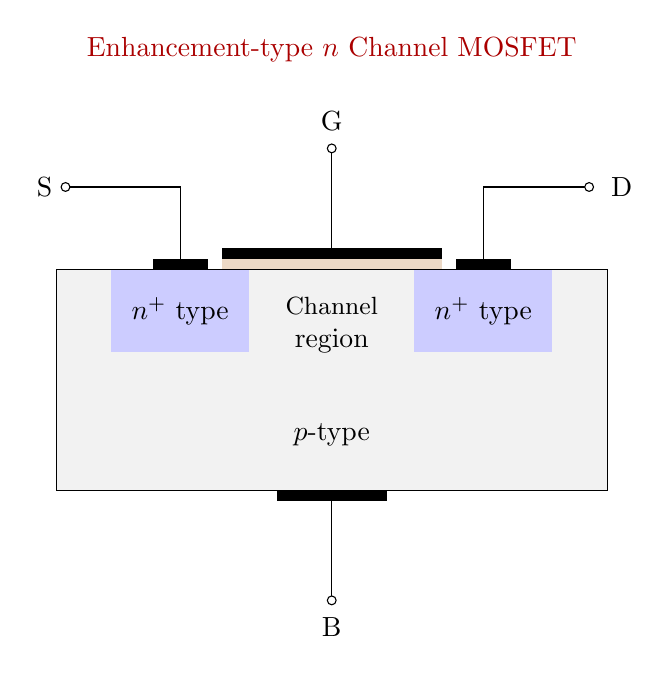
\begin{tikzpicture}
    \begin{scope}[scale=0.7]
        % Title
        \node[anchor=center, color=myred] at (5, 4.0) {Enhancement-type $n$ Channel MOSFET};
        % Regions
        % Substrate
        \fill[gray!10] (0,0) rectangle (10, -4);
        % Source region
        \fill[blue!20] (1, 0) rectangle ++(2.5, -1.5);
        % Source metal contact
        \fill[black] (1.75, 0) rectangle ++(1.0, 0.2);
        % Drain region
        \fill[blue!20] (9, 0) rectangle ++(-2.5, -1.5);
        % Drain metal contact
        \fill[black] (7.25, 0) rectangle ++(1.0, 0.2);
        % Insulated gate region (hased rectangle)
        \fill[brown!30] (3, 0) rectangle ++(4, 0.25);
        \draw[thin, black] (0, 0) rectangle (10, -4);
        % Drain metal contact
        \fill[black] (3, 0.2) rectangle ++(4, 0.2);
        % Body metal contact
        \fill[black] (4, -4) rectangle ++(2, -0.2);
        % Annotate the channel.
        \node[anchor=center, align=center, color=black] at (5, -1.0) {\small Channel\\ region};
        % Wires adn contacts
        % Source
        \draw[black] (2.25, 0) -- ++(0, 1.5) -- ++(-2, 0);
        \draw[ocirc] (0.25, 1.5) node[anchor=east] {};
        \node[anchor=east, color=black, xshift=-0.1cm] at (0.25, 1.5) {S};
        % Drain
        \draw[black] (7.75, 0) -- ++(0, 1.5) -- ++(2, 0);
        \draw[ocirc] (9.75, 1.5) node[anchor=east] {};
        \node[anchor=west, color=black, xshift=0.1cm] at (9.75, 1.5) {D};
        % Gate
        \draw[black] (5.0, 0.2) -- ++(0, 2.0);
        \draw[ocirc] (5.0, 2.2) node[] {};
        \node[anchor=south, color=black, yshift=0.1cm] at (5.0, 2.2) {G};
        % Body
        \draw[black] (5.0, -4) -- ++(0, -2.0);
        \draw[ocirc] (5.0, -6) node[] {};
        \node[anchor=north, color=black, yshift=-0.1cm] at (5.0, -6) {B};

        % Annotate the regions
        \node[anchor=center, color=black] at (2.25, -0.75) {$n^+$ type};
        \node[anchor=center, color=black] at (7.75, -0.75) {$n^+$ type};
        \node[anchor=center, color=black] at (5.0, -3.0) {$p$-type};
    \end{scope}
\end{tikzpicture}
\end{document}